\documentclass{article}
\usepackage{amsmath}
\usepackage{graphicx}
\usepackage{hyperref}
\hypersetup{
		colorlinks=true,
		linkcolor=blue,
		filecolor=magenta,
		urlcolor=cyan,
		pdftitle={Overleaf Example},
		pdfpagemode=FullScreen,
	}
\usepackage{float}
\floatstyle{boxed} 
\restylefloat{figure}
\title{Verilog notes}
\date{01-29-2023}
\author{Tommy Bui}

\begin{document}
	\maketitle
	\newpage
	\pagenumbering{arabic}

	\tableofcontents
	\newpage

	\section{Verilog Tutorial}

	\href{https://www.chipverify.com/verilog/verilog-tutorial}{Reference to Chipverify} \newline

	\subsection{Lore}
	In the early days of integrated circuits, engineers had to physically draw transistors \& their netlist on paper. As circuits became more complex and larger in scale, this process eventually tedious. Languages such as VHDL \& Verilog were developed to simply the process of describing the functionality of IC and let tools convert the behavior into hardware using combinational \& sequential logic. \newline

	\subsection{How is Verilog useful}
	Verilog creates a level of abstraction that hides the details of its implementation \& technology. \newline

	E.g. the design of a D flip-flop requires the knowledge of the transistor layout in order to achieve an edge-triggered FF, rise/setup time, fall/clk-Q times to latch value onto flop, etc.

	\section{Introduction to Verilog}
	\href{https://www.chipverify.com/verilog/verilog-introduction}{Source}

	A digital element such as a FF can be represented using combinational gates such as NAND or NOR gates. The functionality of a FF is determined based on the layout of such gates. \underline{How the gates have to be connected is usually determined using K-maps} \newline

	Below is an schemetic of a Data flip-flop \& its corresponding truth table. The output, q is asserted only when rstn \& d are both set. \newline

	\begin{figure}[H]
		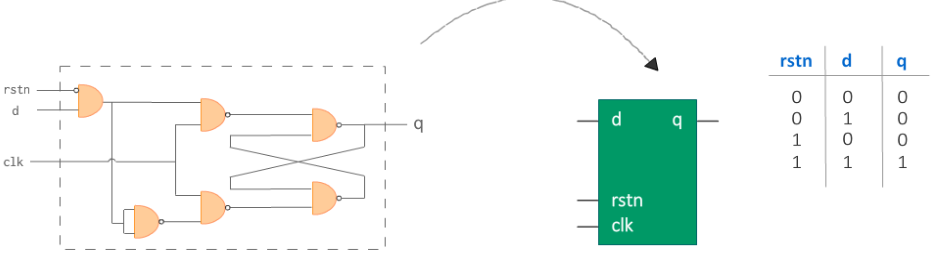
\includegraphics[width=\linewidth]{VerilogPics/figure_1.png}
		\caption{D flip flop}
		\label{D Flip-flop schematic and logic}
	\end{figure}

	\subsection{What is a hardware schematic?}

	A hardware schematic is a daigram that shows how the combinational gates should be connected to implemented a particular behaviour in hardware. From figure 1, a set of NAND gates are connected in order to create a D flip flop. 

	\subsection{What is a Hardware Description Language?}

	It's easier to describe how a block of logic should behave \& let software tools convert that behavior into an actual hardware scchematic. The langugage that describes the hardware functinality is classified as a Hardware Description Language.

	\subsection{Sections of Verilog Code}

	All behavior code should be described within the keywords module \& endmodule. 

	\subsubsection{Verilog section template}
	\begin{itemize}
		\item Module definition \& port list declaration
		\item List of input \& output ports
		\item Declaration of Verilog data types
		\item Module instantiations
		\item Behavioural code
	\end{itemize}

	\begin{figure}[H]
		
\includegraphics[width=\linewidth]{VerilogPics/figure_2.png}
		\caption{Verilog example Template}
		\label{Verilog Template}
	\end{figure}

	\section{Data Types}
	\subsection{Verilog Syntax}

	\href{https://www.chipverify.com/verilog/verilog-syntax}{Source} 
	\href{https://en.wikipedia.org/wiki/Lexical_item}{(Lexical item. In lexicography [citation needed], a lexical item is a single word, a part of a word, or a chain of words ( catena) that forms the basic elements of a language's lexicon (vocabulary)).} \newline \newline

	Lexical conventions in Verilog are similar to C in the sense that it contains a sense of tokens. A lexical token may consist of one or more characters and tokens can be comments, keywords, numbers, strings or white space. However, all lines are terminated by a semi-colon. \newline

	Verilog is case-sensitive, so variables, var\_a \& var\_A differ.


	Two types of comments:
	\begin{itemize}
		\item Single-line comment uses two forward slashes (e.g. //). Single line comments can be nested in a multiple line comment.
		\item Multiple-line comment starts with /* and ends with */ and cannot be nested
	\end{itemize} 
	
	\subsubsection{White space}

	White space refers to spaces, tabs, newlines, \& formfeeds, and is usually ignored by Verilog except when it separates tokens. Be sure to take advantage of this when making readable code. \newline

	\subsubsection{Operators}

	There are three types of operators: unary, binary, \& ternary or conditional. \newline

	\begin{itemize}
		\item Unary operators shall appear to the left of their operand
		\item Binary operators shall appear between their operands
		\item Conditional operators have 2 separate operates that separate 3 operands
	\end{itemize}

	\begin{figure}[H]
		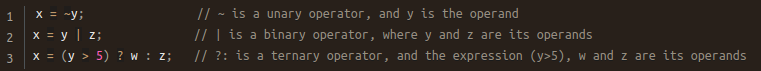
\includegraphics[width=\linewidth]{VerilogPics/figure_3.png}
		\caption{Example of unary, binary, and ternary/conditional operators}
		\label{Example of unary, binary, and ternary/conditional operators}
	\end{figure}

	If the expression (y>5) is true, then variable x will get the value w, else y=z.

	\subsubsection{Number Format}

	\begin{figure}[H]
		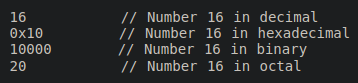
\includegraphics[width=\linewidth]{VerilogPics/figure_4.png}
		\caption{number formats}
		\label{number formats}
	\end{figure}

	By default, Verilog simulators treat numbers as decimals. In order to represent them in different radixes, there are certain rules which must be used. \newline

	\underline{Sized}

	Sized numbers are represented as show below, where size is written only in decimal to specify the number of bits in the number:

	\begin{figure}[H]
		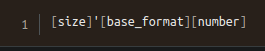
\includegraphics[width=\linewidth]{VerilogPics/figure_5.png}
		\caption{Template for sized numbers}
		\label{Template for sized numbers}
	\end{figure}

	\begin{itemize}
		\item base\_format can be decimal('d or 'D), hex('h or 'H), or octal('o or 'O) \& specifies the base of the number
		\item number can be specified as any valid digit with respect to the specified based format
	\end{itemize}

	\begin{figure}[H]
		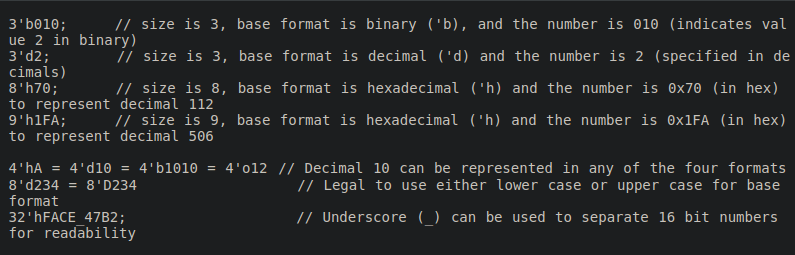
\includegraphics[width=\linewidth]{VerilogPics/figure_6.png}
		\caption{ToDo}
		\label{ToDo}
	\end{figure}

	\subsubsection{Unsized}

	Numbers without a size format specification have a default number of bits depending on the simulator \& machine.

	\subsubsection{Negative} 
	Negative numbers are specified with the - sign before the size of a number; It is illegal to have the - between base format \& number.

	\begin{figure}[H]
		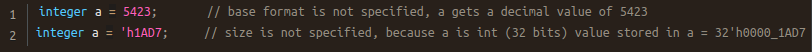
\includegraphics[width=\linewidth]{VerilogPics/figure_7.png}
		\caption{ToDo}
		\label{ToDo}
	\end{figure}
	\subsubsection{Strings} 

	A sequence of characters enclosed in double quotes are strings. It cannot be split into multiple lines \& every chracter in the string takes 1B to be stored:

	\begin{figure}[H]
		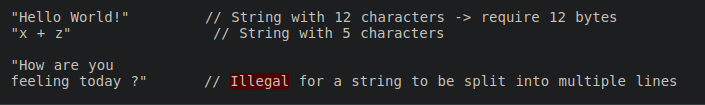
\includegraphics[width=\linewidth]{VerilogPics/figure_8.png}
		\caption{ToDo}
		\label{ToDo}
	\end{figure}
	
	\subsubsection{Identifiers} 

	Identifiers are names of variables; Can be made of alphanumeric characters and symbols. They cannot start with a digit nor a \$:

	\begin{figure}[H]
		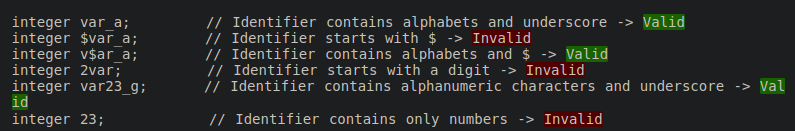
\includegraphics[width=\linewidth]{VerilogPics/figure_9.png}
		\caption{ToDo}
		\label{ToDo}
	\end{figure}

	\subsubsection{Keywords}

	Keywords are special identifiers reserved to be define the language constructs \& are lower case. A list of important keywords is as follows:

	\begin{figure}[H]
		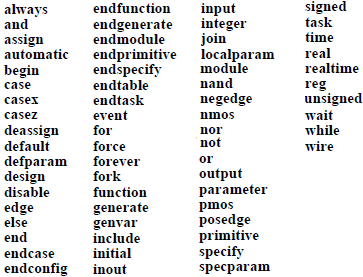
\includegraphics[width=\linewidth]{VerilogPics/figure_10.png}
		\caption{ToDo}
		\label{ToDo}
	\end{figure}

	\subsubsection{Verilog Revisions}
	\begin{figure}[H]
		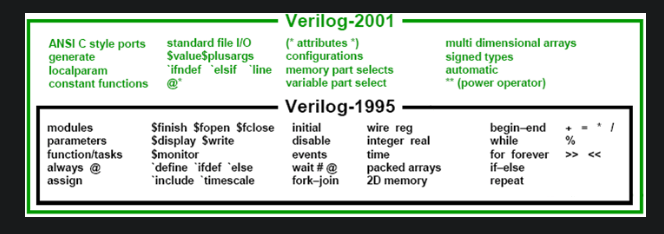
\includegraphics[width=\linewidth]{VerilogPics/figure_11.png}
		\caption{ToDo}
		\label{ToDo}
	\end{figure}




	\subsection{Verilog Data Types}

	\href{https://www.chipverify.com/verilog/verilog-data-types}{Source} \newline \newline

	Data-types in Verilog is meant to represent data storage elements like bits in a flip-flop \& transmission elements like wires that connect between logic gates \& sequential structures. 

	\subsubsection{What values do variables hold?}

	Almost all data-types can have one of the four different values as given below except for \underline{real} \& \underline{event} data types. \newline \newline

	\begin{tabular}{|l|p{6cm}|}
		\hline
		0 & Represents logic zero or false condition \\
		\hline
		1 & Refresents logic one or a true condition \\
		\hline
		x & Represents an unknown logic value (could be 0 or 1, metastability) \\
		\hline
		z & Represents high impedance state \\
		\hline
	\end{tabular}

	The following image shows how these values are represented in timing diagrams \& simulation waveforms. Most simulators use this convention where red stands for X and orange in the middle
	stands for high-impedance or Z. \newline
	:w
	
	\begin{figure}[H]
		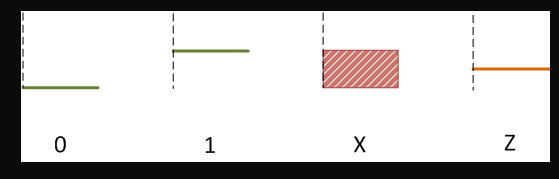
\includegraphics[width=\linewidth]{VerilogPics/figure_12.png}
		\caption{ToDo}
		\label{ToDo}
	\end{figure}

	\subsubsection{What does the verilog value-set imply?}

	Since Verilog is essentially used to describe hardware elements like flip-flops \& combinational logic like NAND \& NOR, it has to model the value system found in hardware. A logic one would
	represent the voltage supply $V_d_d$. \newline \newline

	X or x means that the value is unknown at the time and could either be 1 or 0. This is an issue known as metastability. This differs from the boolean logic X, where it signifies don't care. \newline \newline

	As with any incomplete eletric circuit, the wire that is not connected to anything will have high-impedance at that node which is represented by Z or z. \newline

	\subsubsection{Nets \& Variables}

	Nets \& variables are the two main groups of data types which represent different hardware structures \& differ in the way they are assigned \& retain values. \newline \newline

	\underline{Nets}

	Nets are used to connect between hardware entities like logic gates \& don't store any values on their own. In the follow image, a net\_11 connects between the output of the AND gate and the first
	input of the flip\_floped called data\_0. Similarly, the inputs of the AND gate are connected to nets, net\_45 \& net\_67. \newline

	\begin{figure}[H]
		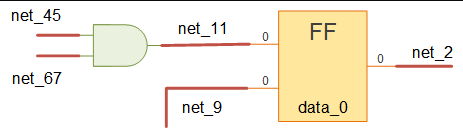
\includegraphics[width=\linewidth]{VerilogPics/figure_13.png}
		\caption{ToDo}
		\label{ToDo}
	\end{figure}

	There are different types of nets with various characterisitcs, the most commonly used net in digital design is of type wire.
Wire is a Verilog data-type used to connect elements \& to connect nets that are driven by a single gate or continuous assignment.

	When there is a requirement for multiple nets, they can be bunched together to form a single wire. In the code below, we can have 
	a 4-bit wire that sends 4 separate values on each one of these wires. A group of such entities is consider a vector. 

	\[ wire [3:0] n0; // 4-bit wire; example of a vector \]

	It is illegal to redeclare a variable name already declared by a net, parameter, or variable. \newline \newline

	\underline{Variables} \newline \newline

	A variable is an abstraction of a data storage element \& can hold values e.g. A flip\-flop. \newline

	Verilog data\-type, reg can be used to model hardware registers since it can hold values between assignments. Note that a reg does not always represent a flip\-flop as it can also represent 
	combinational logic. \newline

	\subsubsection{Other Data\-Types}

	\underline{Integer} \newline \newline 

	\href{https://www.chipverify.com/systemverilog/systemverilog-datatypes}{Properties of data\-types in SV (hopefully same in Verilog)} \newline \newline 

	An integer is a general purpose variable of 32-bits wide which is signed that can be used for other purposes while modeling hardware \& stores integer values.\newline \newline 

	\underline{Time} \newline \newline 

	Time is an unsigned \& 64\-bits wide \& can be used to store simulation time quantities for debugging purposes. A realtime variable simply stores time as a floating point quantity. \newline \newline 

	\underline{Real} \newline \newline

	A real variable can store floating point values \& can be assigned the same way as integer \& reg (See Don Mills' book for properties).

	\subsubsection{Verilog Strings}

	Strings are stored in reg, and the width of the reg variable has to be large enough to hold the string. Each character in a string represents an ASCII value \& requires 1 byte. If the size of the
	variable is smaller than the string, then Verilog truncates teh leftmost bits of the string. If the size of the variable is larger then Verilog appends zeros to the beginning of the string.

	\begin{figure}[H]
		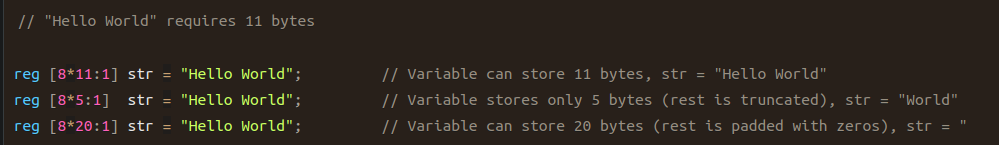
\includegraphics[width=\linewidth]{VerilogPics/figure_14.png}
		\caption{ToDo}
		\label{ToDo}
	\end{figure}



\end{document} 
